\documentclass[titlepage,a4paper, 11pt]{article}

\usepackage[dutch]{babel}
\usepackage{graphicx,fancyhdr,hyperref,a4wide}	
\usepackage{listings}
\lstset{language=C,
basicstyle=\ttfamily\footnotesize,
mathescape=true,
breaklines=true}
\lstset{
  literate={ï}{{\"i}}1
           {ì}{{\`i}}1
}

%\setlength{\parindent}{0.0in}     % inspringen bij nieuwe alinea?
%\setlength{\parskip}{0.1in}       %ruimte laten tussen alinea' s?
%\newcommand{\HRule}{\rule{\linewidth}{0.5mm}}

\newcommand{\mcode}{TIRDES01}  %modulecode
\newcommand{\mname}{Design patterns} %modulenaam
\newcommand{\HRule}{\rule{\linewidth}{1pt}} % dikke horizontale lijn voor frontpagina

\renewcommand{\headrulewidth}{0.4pt}     %dikte van headerlijn
\renewcommand{\footrulewidth}{0.4pt}     %dikte van footerlijn

\headheight = 70pt                        %body van pagina verder naar beneden
\voffset = -40pt                          %corrigeren, anders valt footer van de pagina
\lhead{\large Modulewijzer}               %linker headertekst
\chead{\large Hogeschool Rotterdam}       %centraal headertekst
\rhead{
\includegraphics[width=2cm]{logo}} %rechter headertekst met logo

\lfoot{\mcode\ \today}                    %linker foot tekst: modulecode en datum
\cfoot{}                                  %center foot tekst leeg

\pagestyle{fancy}                         % het fancyheaders pakket van van Oostrum gebruiken


\begin{document}
\sffamily
%%%%%%%%%%%%%%%%%%%%%%%%%%%%FRONTPAGINA%%%%%%%%%%%%%%%%%%%
\begin{titlepage}

\thispagestyle{fancy}
\ \\
\ \\
\ \\
\begin{center}

% Titel
  \textsc{\LARGE Hogeschool Rotterdam / CMI}\\[1.5cm]

  \HRule \\[0.4cm]
  { \Huge \bfseries \mname}\\[0.4cm]
  \ \\
  \ \\
  { \large \bfseries \mcode}\\[0.4cm]

  \HRule \\[1.5cm]

  \vfill
  % Author and supervisor
  \begin{minipage}{0.5\textwidth}
    \begin{flushleft}
      Aantal studieunten: 3 ects\\
      Modulebeheerder: Wessel Oele
    \end{flushleft}
\end{minipage}
\begin{minipage}{0.4\textwidth}
  \begin{flushright}
		\begin{tabular}{ | l l |}
		  \hline
		  Goedgekeurd door: &\ \\
		  \textbf{(namens toetscommissie)} & \ \\
		  Datum: & \ \\
		  \hline
		\end{tabular}
  \end{flushright}
\end{minipage}
\end{center}
\end{titlepage}
%%%%%%%%%%%%%%%%%%%%%%%%%%%%FRONTPAGINA%%%%%%%%%%%%%%%%%%%
\rfoot{\thepage} %pagina nummering vanaf inhoudsopgave
\tableofcontents %inhoudsopgave
\newpage
%%%%%%%%%%%%%%%%%%%%%%%%%%%%MODULE A4-TJE%%%%%%%%%%%%%%%%%
\section*{Modulebeschrijving}
\scriptsize
\begin{tabular}{|p{3cm}|p{11cm}|}
\hline
Modulenaam:&\mname\\
\hline
Modulecode:&\mcode\\
\hline
Aantal studiepunten en studiebelastingsuren:&Deze module levert 3 studiepunten op.
\begin{itemize}
\item 8 $\times$ 120 minuten hoorcollege
\item 8 $\times$ 120 minuten practicum
\item 12 $\times$ 120 minuten zelfstudie
\end{itemize}
\\
\hline
Vereiste voorkennis:&Java: basis, o.o.p., toepassen, datastructuren\\
\hline
Werkvorm:&hoorcollege en practicum\\
\hline
Toetsing:&Practicumopdrachten\\
\hline
Leermiddelen:&Design patterns explained, auteur: Alan Shalloway, James R. Trott, uitgever: Addison Wesley, ISBN: 978-0-321-24714-8\\
\hline
Draagt bij aan competentie&\begin{center}
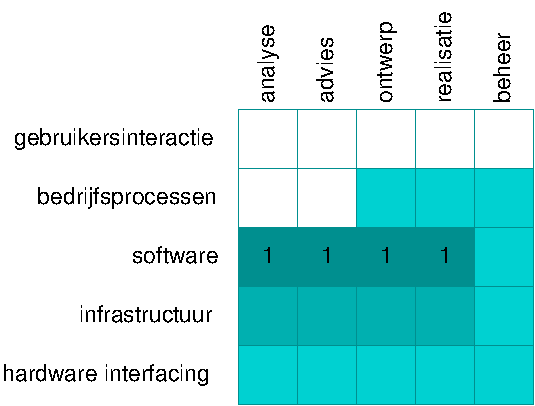
\includegraphics[width=7cm]{comptabel}
\end{center}\\
\hline
Leerdoelen:&Kunnen werken met U.M.L. Begrijpen en kunnen toepassen van diverse design patterns zoals adapter, facade, bridge, abstract factory, e.v.a.\\
\hline
Inhoud:&
\begin{itemize}
\item U.M.L.
\item Diverse design patterns
\end{itemize}\\
\hline
Opmerkingen:&\\
\hline
Modulebeheerder:&Wessel Oele\\
\hline 
Datum:&\today\\
\hline
\end{tabular}
%%%%%%%%%%%%%%%%%%%%%%%%%%%%MODULE A4-TJE%%%%%%%%%%%%%%%%%
\newpage
\normalsize
\section{Algemene omschrijving}
Het correct ontwerpen van software is een gecompliceerde zaak. Niet alleen is het ontwerpen zelf niet eenvoudig, moeilijker wordt het wanneer de eisen, waaraan een stuk software moet voldoen ook nog eens veranderen. Ten slotte zijn de meeste computerprogramma' s nooit af en dient er in de jaren na oplevering met enige regelmaat aan onderhoud en uitbreiding gedaan te worden. 

Design patterns vormen een hulpmiddel bij het ontwerpen van software, opdat software zo ontworpen kan worden dat het aanpassen en uitbreiden van de software eenvoudiger wordt. Ook vergroot het gebruik van design patterns de herbruikbaarheid van (delen van) de software.

Design patterns vinden hun oorsprong in het einde van de jaren '70 toen Christopher Alexander patronen als hulpmiddel gebruikte bij het ontwerpen van gebouwen en steden. Na enig experimenteel werk van Beck en Cunningham werden design patterns populair in de jaren '90 toen de zogeheten ``gang of four'' (Erich Gamma, Richard Helm, Ralph Johnson en John Vlissides) het boek \emph{``Design Patterns: Elements of Reusable Object-Oriented Software''} publiceerden.
\subsection{Relatie met andere onderwijseenheden}
Deze module bouwt voort op de modules tinpro01-1, tinpro01-2, tinpro01-3, en tinpro01-4. Verondersteld wordt het programmeren in een imperatieve en objectgeori\"enteerde taal te beheersen. 
\subsection{Leermiddelen}
Verplicht:
\begin{itemize}
\item Boek: Design patterns explained, auteur: Alan Shalloway, James R. Trott, uitgever: Addison Wesley, ISBN: 978-0-321-24714-8
\item Software: Java Development Kit (JDK) versie 6, te downloaden van \url{http://www.javasoft.com}
\item Presentaties die gebruikt worden in de hoorcolleges (pdf): te vinden op \url{http://med.hro.nl/oelew}
\item Opdrachten, waaraan gewerkt wordt tijdens het practicum (pdf): te vinden op \url{http://med.hro.nl/oelew}
\end{itemize}
Facultatief:
\begin{itemize}
\item Boek: Design Patterns: Elements of Reusable Object-Oriented Software, auteur: Gamma, Helm, Johnson, Vlissides ,uitgever: Addison-Wesley. ISBN 0-201-63361-2
\item Text editors: Emacs, VI, Jedit, Gedit, etc.
\end{itemize}

\section{Programma}

\begin{tabular}{|p{1cm}|p{4cm}|p{4cm}|}
\hline
Week&Literatuur&Lesinhoud\\
\hline
1&D.P. Explained t/m blz. 45,&introductie, herhaling o.o.p., u.m.l.\\
\hline
2&D.P. Explained t/m blz. 73&o.o.p. problemen\\
\hline
3&D.P. Explained t/m blz. 115&facade en adapter pattern\\
\hline
4&D.P. Explained t/m blz. 136&denkwijze en perspectief\\
\hline
5&D.P. Explained t/m blz. 157&strategy pattern\\
\hline
6&D.P. Explained t/m blz. 191&bridge pattern\\
\hline
7&D.P. Explained t/m blz. 212&abstract factory pattern (inleveren groepsopdrachten bij practicum)\\
\hline
8&D.P. Explained t/m blz. 266 &\\
\hline
9&&vragenuur/inhaalles\\
\hline
10&&vragenuur/inhaalles\\
\hline
\end{tabular}
\section{Toetsing en beoordeling}
Twee procedures zijn, afhankelijk van de opdracht en docent, beschikbaar:

\subsection{Procedure 1}
Deze module wordt getoetst middels groepsopdrachten. Voorwaarden:
\begin{itemize}
\item Opdrachten worden op papier en tijdens de practicumlessen ingeleverd.
\item Een groep bestaat uit maximaal vier studenten. Deze leveren gezamenlijk \'e\'en opdracht in.
\item Bij het inleveren zijn alle leden van de groep aanwezig, opdat \emph{elk} lid de uitwerking mondeling kan verdedigen.
\item De practicumdocent kan naar eigen inzicht (bijvoorbeeld om didactische redenen) afwijken van de practicumopgaven en alternatieve opdrachten aanbieden. Hierbij staat duidelijkheid en integriteit richting de studenten uiteraard voorop.
\end{itemize}


\subsection{Procedure 2}
The module is examinated through a series of heavily connected practicum assignments. The assignment feature the building of a simple game in a modern mainstream OO language such as Java or C\#. The assignments will begin with an unstructured, mostly procedural game which, through the application of design patterns, will become always more structured. The parts of the game will become more and more independent from each other, and at the same time more reusable.

Handing in is done through GitHub, with a project with name 

\texttt{MODULE-CODE\_STUDENT-NUMBER1\_STUDENT-NUMBER2\_STUDENT-NUMBER3\_STUDENT-NUMBER4}. 

Therefore, a group made up of students 123456, 654321, 123654, and 654123 would hand-in a public GitHub project with name:

\texttt{TIRDES01\_123456\_654321\_123654\_654123}.

At the worst weekly check-ins will be required \textit{from every member of the team}. Even though the course allows group work, delegation is not permitted. Each and every member of the team \textbf{must know} how all aspects of the handed-in code work. This will be ascertained through an oral check (\textbf{not an oral examination}) where students will be asked to explain random parts of the code, independently from authorship.

\textbf{The oral check will be done during the last practicum lecture, which is also the final deadline. During the last lecture grades will be given.} Retake will happen following the same examination structure: a short oral check based on the handed-in GitHub project. Retake will be done during the exam weeks of the second period.

\paragraph*{Assignment 0 - the basics}
The first assignment requires building a very small game. For the assignment to be sufficient, the game must feature at the very least:
\begin{itemize}
\item at least three different entities with different roles within the game (for example spaceships, asteroids, and projectiles)
\item input in order to control some entities (for example the keys to move the spaceship and the space key to shoot projectiles)
\item interaction between entities (for example contact between projectiles and asteroids causes both to disappear and an explosion to take place)
\end{itemize}

It is highly recommended to use the combination of C\# and the open-source software MonoGame in order to build the game. Similar environments do exist in Java and may be used. For an extra challenge (and therefore extra points), other languages which may be used are F\# and Haskell.

\textbf{Score: 25\%}


\paragraph*{Assignment 1 - adapter/façade for rendering}
Separate the game logic and the rendering logic through a mixture of façade (the rendering system) and adapters (for the objects to render). The main representation of data is done in the game-logic object, whereas the adapters store additional, rendering-specific data.

\textbf{Score: 25\%}


\paragraph*{Assignment 2 - factory and abstract factory}
Factor out the logic for the creation of objects (and their rendering adapters) within a list of abstract factories that determine themselves when and how to create objects for the game logic and rendering façade.

\textbf{Score: 25\%}


\paragraph*{Assignment 3 - strategy/decorator}
Build a series of classes that implement the interface:

\begin{lstlisting}
interface Script {
  bool Tick(float dt);
  Script Reset();
}
\end{lstlisting}

Concrete implementations of the class will be, at the very least:
\begin{itemize}
\item the \texttt{Wait} class, which \texttt{Tick} method returns \texttt{true} only after a certain amount of time
\item the \texttt{WaitKeyPress} class, which \texttt{Tick} method returns \texttt{true} only after a certain key is pressed
\item the \texttt{Sequentialize} class, which \texttt{Tick} method returns \texttt{true} only after all its internal \texttt{Script} instances have returned \texttt{true}, in the proper storage order
\item the \texttt{Repeat} class, which \texttt{Tick} method always returns \texttt{false} but, whenever the internal \texttt{Script} is done (its \texttt{Tick} method returns \texttt{true}), invokes \texttt{Reset} on the internal \texttt{Script} to start it again
\end{itemize}

\textbf{Score: 25\%}

\newpage
\section{Bijlage 1: Toetsmatrijs}
\begin{tabular}{|p{1cm}|p{4cm}|p{4cm}|p{4cm}|}
\hline
&Leerdoelen&Dublin descriptoren&Verwijzing naar opdracht / vraag / criteria\\
\hline
1&o.o.p., u.m.l.&1,2,3,4&practicumopdracht 1 \\
\hline
2&adapter, facade&1,2,3,4&practicumopdracht 2 \\
\hline
3&abstract factory&1,2,3,4&practicumopdracht 3\\
\hline
4&strategy/decorator&1,2,3,4&practicumopdracht 4\\
\hline
\end{tabular}\\
\vspace{1cm}\\
Dublin-descriptoren:
\begin{enumerate}
\item Kennis en inzicht
\item Toepassen kennis en inzicht
\item Oordeelsvorming
\item Communicatie
\end{enumerate}
\newpage

\section{Bijlage 3: Studielast (normering in ecs)}
\begin{tabular}{|l|p{3cm}|p{3cm}|p{2cm}|}
\hline
&aantal weken&aantal lesuren van 50 minuten&klokuren\\
\hline
\emph{lesuren}&10&4&33\\
\hline
&&&\\
\hline
\emph{zelfstudie}&&&\\
\hline
&&&\\
\hline
leestijd&aantal pagina' s&&\\
\hline
&& 3 per uur&\\
\hline
&& 6 per uur&\\
\hline
&120& 10 per uur&12\\
\hline
&&&\\
\hline
presentaties&&&\\
\hline
&&&\\
\hline
overlegtijd&&&\\
\hline
&&&\\
\hline
uitzoektijd/research&&&11\\
\hline
&&&\\
\hline
niet ingeroosterde lestijd&&&\\
\hline
&&&\\
\hline
\emph{toetsen}&voorbereiden&&3.5\\
\hline
&toets&&1.5\\
\hline
&nabespreking&&1\\
\hline
&&&\\
\hline
\emph{werkstuk,verslag,rapport,scriptie}&uitzoeken&&\\
\hline
&overleggen&&\\
\hline
&schrijven&&\\
\hline
&&&\\
\hline
Stage, Praktijkopdracht&voorbereiding&&\\
\hline
&aanwezigheid&&\\
\hline
&overleg&&\\
\hline
&&&\\
\hline
\emph{Subtotaal in klokuren}&&&56\\
\hline
\emph{Ruis 5\%}&&&\\
\hline
\emph{Totaal in klokuren}&&&56\\
\hline
\emph{Totaal in studiepunten (ects)}&&&2\\
\hline
\end{tabular}
\end{document}


